\section{Cambios con respecto al diseno}
\label{sec:CambiosConRespectoAlDiseno}

\begin{itemize}
	\item No realizamos grandes cambios conceptuales a sobre lo que habiamos dise�ado, esto nos fue de ayuda a la hora de modularizar el trabajo.
	\item Uno lo de los cambios fue separar la responsablidad de la mesa de craps de fotografiarse, como lo hacia en el dise�o y agregamos un visitor para que se encargara de esta tarea.
	\item Los mensajeros cambiaron un poco tambien dado que potencialmente podian llegar a tener que trabajar todos en la misma carpeta, por lo que debian tener algun tipo de filtro que les permitiera distinguir los archivos que le tocaban de los que no le tocaban. Tambien como el servidor debia correr a todos los mensajeros al mismo tiempo debimos lanzarlos en threads diferentes.
	\item Descubrimos un poco tarde la eleccion poco feliz de la representacion de los mensajes del casino que termino generando mas acoplamiento del que creiamos.
	\item Al encontrar problemas complejos en algunas clases fuimos delegando algunas responsablilidades a clases nuevas como por ejemplo en ManejdorDeSaldo y el ManejadorDeApuestas.
\end{itemize}

\subsection{Dependencias}
\label{sec:Dependencias}

Logramos que las dependencias resultaran como las previstas, exepto por las dependencias del ``lanzador del casino''.

\begin{figure}[htbp]
	\centering
		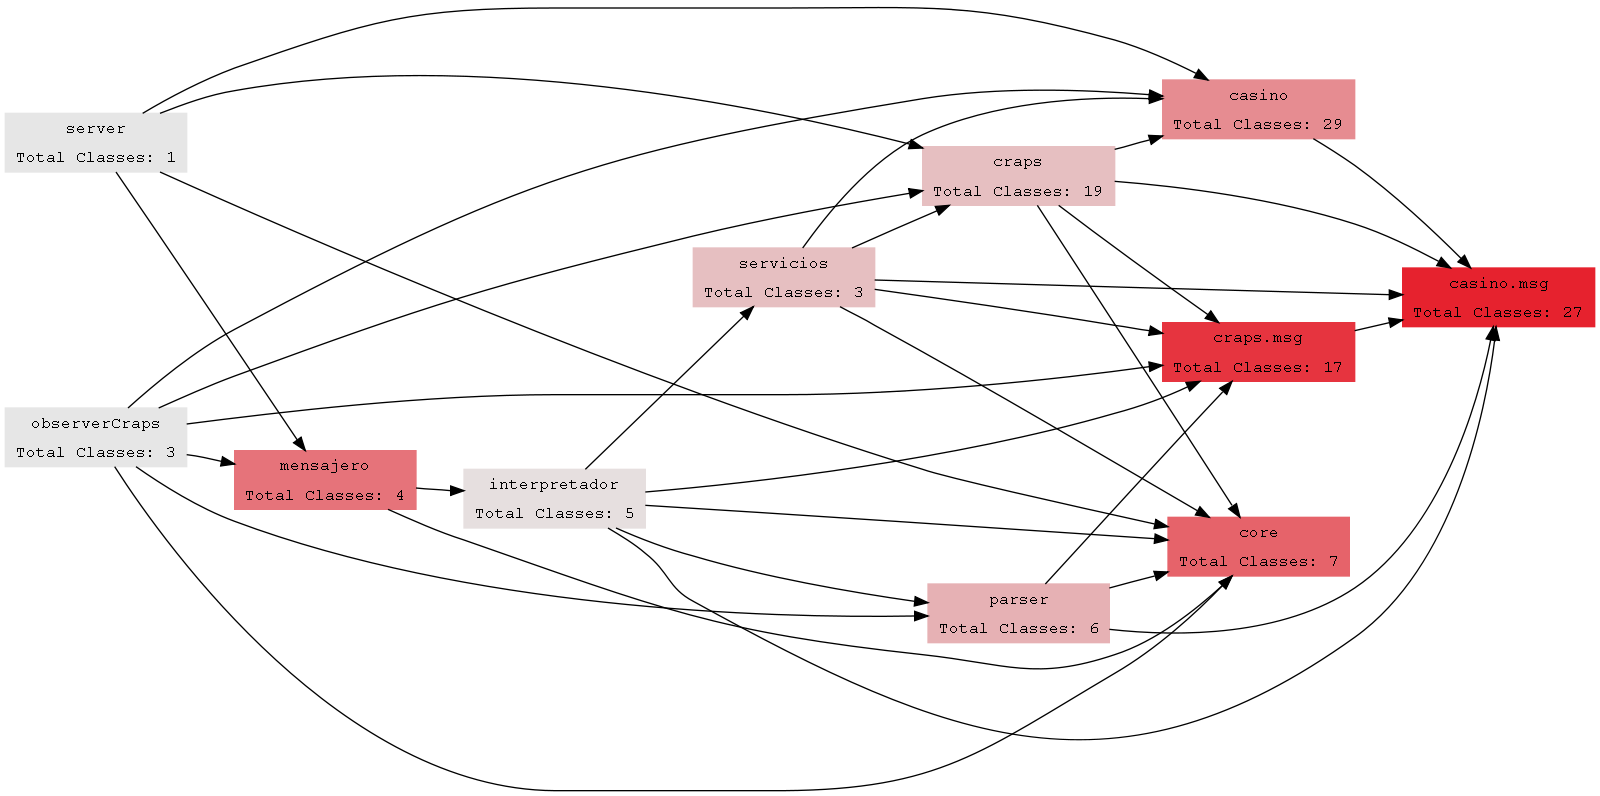
\includegraphics[width=1.00\textwidth]{img/jdepend-report.png}
	\label{fig:jdepend-report}
\end{figure}


